\begin{fquestion}{Was ist Symmetriebrechung?}
    Symmetriebrechung beschreibt den Übergang eines System von einem ungeordneten Zustand hoher Symmetrie in einen in dem die Symmetrie nicht mehr gilt, also gebrochen ist.
    Man kann zwischen kontinuierliche Symmetrien (Drehungen) und diskrete Symmetrien (Spiegelung) unterscheiden.
\end{fquestion}


\begin{fquestion}{Was ist spontane Symmetriebrechung?}
    Bei der spontanen Symmetriebrechung hat der Grundzustand eine andere Symmetrie als das Gesamtsystem (die Bewegungsgleichung). 
    Nimmt das System den Grundzustand ein, wird dadurch dessen Symmetrie ``spontan'' gebrochen.
\end{fquestion}

\begin{fquestion}{Wie hängen Symmetriebrechung und Phasenübergänge allgemein zusammen?}
    Eine Symmetriebrechung impliziert einen Phasenübergang, die Umkehrung gilt nicht.
    Ein Beispiel dafür ist der flüssig-gasförmig Übergang bei Wasser; die Flüssigkeit hat genauso viele Symmetrien wie das Gas.
\end{fquestion}

\begin{fquestion}{Was sind Beispiele von spontaner Symmetriebrechung?}
    Beispiele verschiedener Symmetriebrechungen sind in \autoref{tab:symmetriebrechungen} dargestellt.
\end{fquestion}

\begin{table}[htb]
    \centering
    \begin{tabular}{|llllll|}
        \hline
        \textbf{Phänomen} & Gebrochene & Brechungs- & Ordnungs- & Massive & Goldstone-  \\
        & Symmetrie & parameter & parameter & Anregung & Boson \\
        \hline
        \textbf{Elastischer} & $O(2)$ & Kraft & Biegung & Schwingung & Drehung \\
        \textbf{Stab} & Rotation & & & & \\
        & \multicolumn{5}{l|}{\textit{Keine explizite Symmetriebrechung}} \\
        \hline
        \textbf{Supraleitung} & U(1) & Temperatur, & Cooperpaar- & Schmid-Gap- & massive \\
        & Phasenrotation & Magnetfeld & dichte & Fluktuationen & Anderson- \\
        & & & & & Bogoliubov \\
        &\multicolumn{5}{l|}{\textit{Explizite Symmetriebrechung durch Coulomb-Wechselwirkung}} \\
        \hline
        \textbf{Ferromagne-} & $O(3)$ & Temperatur & Magnetisie- & Spinflip, & Spinwelle  \\
        \textbf{tismus} & Rotation & & rung & Spinwelle & $\lambda = \infty$ \\
        &\multicolumn{5}{l|}{\textit{Explizite Symmetriebrechung durch ein externes Magnetfeld}} \\
        \hline 
        \textbf{Kerndefor-} & $O(3)$ & Valenznu- & Deformation & Asymmetri- & - \\
        \textbf{mation} & Rotation & kleonenzahl & & sche & \\
        & &  & & Vibration & \\
        &\multicolumn{5}{l|}{\textit{Explizite Symmetriebrechung durch magnetische Wechselwirkungen}} \\
        \hline
        \textbf{Hadronen-} & $SU(2)_A$ & Stärke der & $q\bar{q}$- & $\sigma$-Meson & 3 Pionen \\
        \textbf{massen} & Chiral-axial & Ww. & Kondensat & & \\
        & \multicolumn{5}{l|}{\textit{Explizite Symmetriebrechung durch nackte $q$-Masse}} \\
        \hline
        \textbf{Teilchen-} & $SU(2)_L$ & Temperatur & Higgsfeld & Higgsboson & Massive \\
        \textbf{massen} & Elektro- & & ($v = $& & Eichbosonen \\
        & schwach & & $\SI{246}{\giga\electronvolt}$ & &\\
        & \multicolumn{5}{l|}{\textit{Keine explizite Symmetriebrechung}} \\
        \hline
    \end{tabular}
    \caption{Überblick über verschiedene Symmetriebrechungen. Inhaltlich aus dem Vorlesungsskript entnommen.}
    \label{tab:symmetriebrechungen}
\end{table}

\begin{fquestion}{Mit welchen Größen beschreibt man Symmetriebrechung?}
    Man nutzt Ordnungsparameter und Brechungsparameter:
    \begin{itemize}
        \item Der \textit{Ordnungsparameter} ist ein Maß für die Ordnung in einem System. Beim Übergang (Symmetriebrechung, Phasenübergang) von einem Zustand hoher Symmetrie (Unordnung) zu einem niedriger Symmetrie (entsprechend hoher Ordnung) nimmt er anstatt $0$ einen endlichen Wert an.
        
        Auch bei Phasenübergängen ohne Symmetriebrechung nennt man den entsprechenden Parameter Ordnungsparameter.
        \item Der \textit{Brechungsparameter} beschreibt als Größe die Nähe zum Übergang. Erreicht diese einen kritischen Wert, so ist die Symmetrie instabil.
    \end{itemize}
\end{fquestion}

\begin{fquestion}{Wie verhält sich der Ordnungsparameter in Abhängigkeit vom Brechungsparameter mit externem Feld?}
    Passiert der Brechungsparameter einen kritischen Wert, ändert sich der Ordnungsparameter zwischen Null und einem endlichen Wert.

    Wird die Symmetrie durch ein zusätzliches externes Feld explizit gebrochen (beim Beispiel des Ferromagneten durch ein externes Magnetfeld) weicht der Übergang des Ordnungsparameters auf.
    \begin{center}
        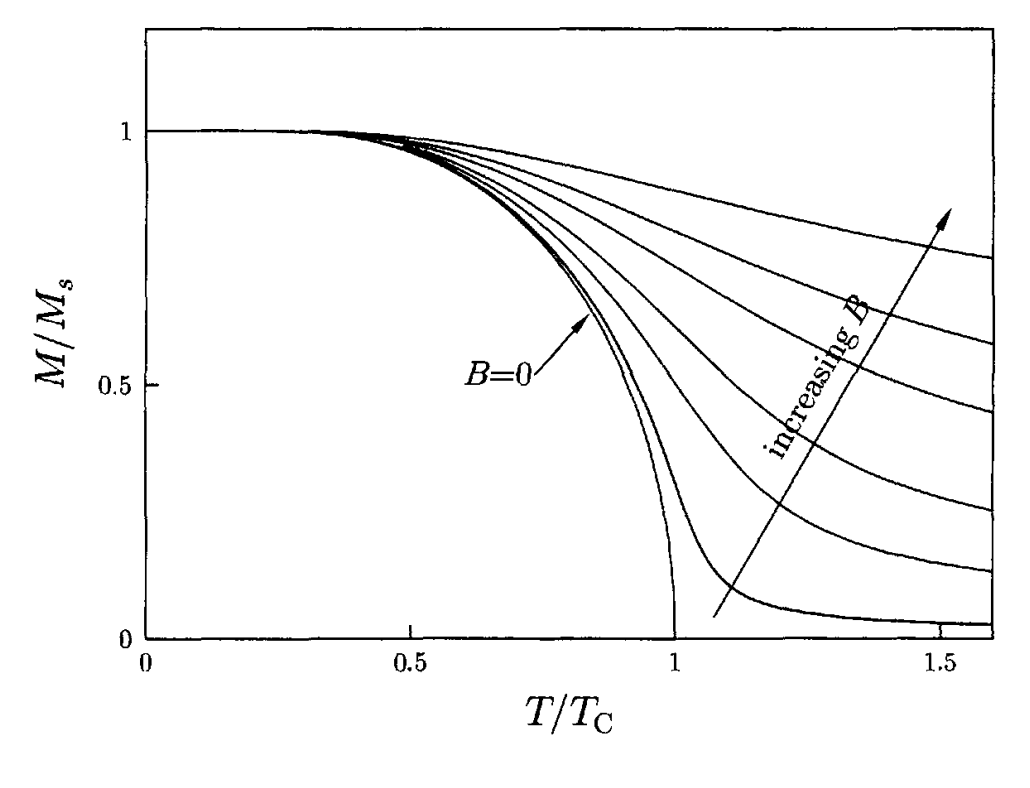
\includegraphics[width=.7\linewidth]{img/Ordnungsparam_Ext_Feld.png}
    \end{center}
    \refimgsourcebook{Magnetism In Condensed Matter (Oxford Master Series In Physics)}{Stephen Blundell}{978-0198505914}{90}
\end{fquestion}

% \begin{question}{Wie können wir die Symmetrie des Systems darstellen und die spontane Symmetriebrechung richtig beschreiben? }
%     Im ungebrochenen Zustand Parabelpotential gemalt (zuerst 2D, dann aber auch 3D erklärt), dann Übergang zum Doppelmuldenpotential erklärt als die Symmetriebrechung, gezeigt, wo sich im Potential der Grundzustand befindet und wie dieser sich ändert
% \end{question}

\begin{fquestion}{Was ist das Coleman-Theorem?}
    Das Coleman-Theorem dient zur Klassifizierung von Symmetriebrechungen.

    Gegeben sei ein quantenmechanisches System mit einer Lagrangedichte $\mathcal{L}$ und einem Zustand minimaler Energie, dem Vakuumzustand.
    Wirkt eine definierte Symmetrietransformation $U$ auf die Lagrangedichte $\mathcal{L}$ oder den Vakuumzustand, treten folgende Fälle auf:
    \begin{enumerate}
        \item Vakuumzustand und $\mathcal{L}$ sind invariant $\implies$ Exakte Symmetrie
        \item Vakuumzustand ist nicht invariant und
        \begin{enumerate}
            \item  $\mathcal{L}$ ist nicht invariant $\implies$ Explizite Symmetriebrechung
            \item $\mathcal{L}$ ist invariant  $\implies$ Spontane Symmetriebrechung
        \end{enumerate}
    \end{enumerate}
\end{fquestion}

\begin{fquestion}{Was ist das Goldstone-Theorem?}
    Die spontane Brechung globaler, kontinuierlicher Symmetrien hat zur Folge, dass zu jedem gebrochenen Generator der Symmetriegruppe ein masseloses skalares Teilchen entsteht.
    Vorstellen kann man sich dies als Anregung in Richtung der Symmetrie, für die eine zur Null fallende Dispersionsrelation gelten muss.
    Das entsprechende Quasiteilchen heißt Nambu-Goldstone-Boson, oder auch Goldstone-Boson.
\end{fquestion}

\subsection{Landau-Theorie}

\begin{fquestion}{Können wir Symmetriebrechung mathematisch beschreiben? }
    Ja, wir zum Beispiel mit der Landau-Theorie. 
    Dafür entwickeln wir das chemische Potential $F(T, \eta)$ in kleinen Ordnungsparametern (also nahe dem Phasenübergang):
    \[F(T, \eta) = F_0 + a(T) \eta^2 + \frac{b(T)}{2} \eta^4 + \mathcal{O}(\eta^6).\]
    Wir vernachlässigen die ungeraden Potenzen unter der Annahme, dass das System unter der Parität $\eta \rightarrow -\eta$ symmetrisch ist; natürlich muss diese Annahme nicht zwingend gelten.
    
    Aus $\partial F / \partial \eta = 0$ als angenommenen Zustand erhalten wir
    \[\eta^2 = - \frac{a(T)}{b(T)}.\]
    Außerdem fordern wir, dass wir uns in einem Potentialminimum befinden und damit $\partial^2 F / \partial^2 \eta = 2 a(T) + 6 b(T) \eta^2 > 0$.
    Hiermit folgt dass $a(T)$ bei $T=T_C$ einen Vorzeichenwechsel hat und die Näherung $a(T) = A (T - T_C)$ sinnvoll ist, $b(T) = B$ wird als konstant angenommen.
\end{fquestion}

\begin{fquestion}{Wieso ist der Parameter $a(T) < 0$ für $T < T_C$? }
    Damit sowohl Ordnungsparameter und zweite Ableitung der freien Energie als auch bspw. Entropie $S = \partial F / \partial T = S_0 - a Q^2$ und spezifische Wärmekapazität $C_p = T (\partial S / \partial T) = C_{p 0} + a^2 T_C/2 B$ (in der Hochtemperaturphase) sinnvoll positiv definiert sind.
\end{fquestion}

\begin{fquestion}{Welche Phasen gibt es in der Landautheorie?}
    \begin{minipage}{\linewidth}
        \begin{table}[H]
            \centering
            \begin{tabular}{|c|c|c|l|}
                \hline
                \textbf{Ordnungspar.} & \textbf{Koeffizienten} & \textbf{Temperatur} & \textbf{Phase} \\
                \hline
                $Q = 0$ & $A > 0$ & $T > T_C$ & Hochtemperaturphase \\
                \hline
                $Q = 0$ & $A = 0$ & $T = T_C$ & Phasenübergangspunkt \\
                \hline
                $Q^2 = -\frac{A}{B}$ & $A < 0, B > 0$ & $T < T_C$ & Tieftemperaturphase \\
                \hline
            \end{tabular}
        \end{table}
    \end{minipage}
\end{fquestion}

\begin{fquestion}{Wie kann man Phasenübergänge erster Ordnung in der Landau-Theorie beschreiben?}
    Wir führen zusätzlich einen Term $C \eta^6$ ein und können damit eine dreibäuchige freie Energie modellieren.
\end{fquestion}

\begin{fquestion}{Wie modelliert eine explizite Symmetrieänderung in der Landau-Theorie?}
    Durch einen zusätzlichen Term $h \eta$ linear im Ordnungsparameter.
\end{fquestion}




\subsection{Ferromagnetismus}

% Wichtig zu wissen ist die Curie-Temperatur $T_C = ?$ und dass die Magnetisierung als Ordnungsparameter fungiert.

\begin{fquestion}{Wie ist das mit der spontanen Symmetriebrechung, wenn ein äußeres Feld angelegt wird? }
    Sie tritt dann gar nicht auf, weil die Symmetrie schon explizit gebrochen wurde.
\end{fquestion}

% \begin{question}{Wie bekommt man einen Phasenübergang erster Ordnung?}
%     Term 6. Ordnung einführen 
% \end{question}

\begin{fquestion}{Was passiert wenn man die Symmetrie explizit bricht durch externes Magnetfeld?}
    Bei Landau Theorie durch Hinzufügen eines linearen Terms beschrieben. 
    
    Es findet kein Phasenübergang mehr statt. 
    
    Die Magnetisierung geht nicht auf Null runter sondern nähert sich nur mit 1/T an.
    
    Bei positiver Suszeptibilität, Paramagnet, wird das äußere Magnetfeld verstärkt. Bei negativer Suszeptibilität, Diamagnet, ist es umgekehrt. 
\end{fquestion}

% \begin{question}{Wie sieht die Magnetisierung bei endlichem Feld aus?}
%     bei hohen Feldern exponentiell unterdrückt
% \end{question}

\begin{fquestion}{Was haben ferromagnetische und chirale Symmetriebrechung gemeinsam?}
positive Rückkopplung, beispielsweise wird eine endliche Magnetisierung bis zur Sättigung verstärkt, dadurch, dass sich die Magnetisierung selbst beeinflusst. 
\end{fquestion}

\begin{fquestion}{Was gibt es für Anregungen im Ferromagneten?}
    Die Anregungen heißen Spinwellen, ihre Quasiteilchen heißen Magnonen.
\end{fquestion}

% \begin{question}{Sie hatten doch erwähnt, dass das auch von der Temperatur abhängig ist, wo steckt denn die T-Abhängigkeit? }
%     Im $a$-Faktor, s.d. $a=a_0(T-T_C)$
% \end{question}

% \begin{question}{Wie sieht dann denn die Energie für $T>Tc$ und $T<Tc$, Mexican-Hat in 2D für TTc nicht auf Null) ??? }
% \end{question}

\begin{fquestion}{Kein Knick mehr, was hat man an dem Knick denn erkannt?  }
    Phasenübergang 2. Ordnung ist, also eine Unstetigkeit in der ersten Ableitung. 
\end{fquestion}

% \begin{question}{Und was bedeutet das dann für die explizite Symmetriebrechung?}
%     Da hier kein Knick ist, ist es auch kein Phasenübergang mehr
% \end{question}

% \subsection{Ordnungsparameter und Brechungsparameter}

% \begin{question}{Wie ändert sich der Verlauf bei Existenz einer äußeren Feldes?}
%     An der kritischen Temperatur ist kein Knick, sondern ein abklingender Verlauf
% \end{question}

% \begin{question}{Wie ändert sich der Verlauf mit steigender äußerer Feldstärke?}
%     Der Bereich, in dem der Graph abfällt, verschiebt sich hin zu höheren Temperaturen
% \end{question}

% \begin{question}{Sind Symmetriebrechung und Phasenübergänge equivalent?}
%     Nein, Symmetriebrechung impliziert Phasenübergang, die Umkehrung gilt aber nicht
% \end{question}


\subsection{Higgs-Mechanismus}

Wichtig zu wissen sind die Lagrangedichte, Potential und Temperaturabhängigkeit.

\begin{fquestion}{Wie ist die Lagrangedichte des Higgsfeldes?}
    Es ist 
    $$\mathcal{L}(\phi) = (\partial_\sigma \phi)^\dagger (\partial^\sigma \phi) + \mu^2 \phi^\dagger \phi - \lambda (\phi^\dagger \phi)^2$$
    die Lagrangedichte des Higgsfeldes.
    Wir identifizieren das Potential
    $$\mathcal{V}(\phi) = -\mu^2 \phi^\dagger \phi + \lambda (\phi^\dagger \phi)^2,$$
    wobei $\mu = \SI{88.45}{GeV/c^2}$ eine Masse und $\lambda = 0.12907$ einheitenlos sind.
\end{fquestion}

\begin{fquestion}{Wie kommt es hier durch spontane Symmetriebrechung zum Massengewinn?}
    Wir betrachten als Modell das skalare Potential 
    $$V(\varphi) = -\mu^2 \varphi^2 + \lambda \varphi^4,$$
    welches sein Minimum bei dem sogenannten Vakuumerwartungswert
    $$\varphi_0 \equiv v = \pm \sqrt{\frac{\mu^2}{2\lambda}}$$
    hat.
    
    Wir entwickeln das ``Feld'' um den Grundzustand mit $\varphi \equiv v + H$ und erhalten
    $$V'(\varphi = v + H) = -\lambda v^4 + 4 \lambda v H^3 + 2 \mu^2 H^2 + \lambda H^4 = V_0 + 2 \mu^2 H^2 + \mathcal{O}(H^3),$$
    wobei das Higgsteilchen eine Masse $\frac{1}{2} m_H^2 = 2 \mu^2$ hat.
    Analog zum Klein-Gordon Feld beschreiben die $\mathcal{O}(H^3)$-Terme Wechselwirkung.
    
    In der komplexen Feldtheorie treten hierbei zwei Felder $h$ und $\chi$ auf, die Lagrangedichte lautet dann
    $$\mathcal{L}_{\mathrm{Higgs}}'(h, \chi) = \frac{1}{2} \partial_\sigma h \partial^\sigma h - \mu^2 h^2 + \frac{1}{2} \partial_\sigma \chi \partial^\sigma \chi + \mathrm{Wechselwirkungen}$$
    wobei das Higgsteilchen die Mase $m_hj = \sqrt{2} \mu$ und das $\chi$-Feld ein masseloses Nabu-Goldstone-Boson ist.
    
    Koppelt nun das Higgsfeld über
    $$\partial^\sigma \rightarrow D^\sigma = \partial^\sigma - i g A^\sigma$$
    an das Eichfeld $A^\sigma$ entsteht in der Lagrangedichte ein Term
    $$\mathcal{L}(A, h, \chi) = \frac{g^2 v^2}{2} A_\sigma A^\sigma + \ldots,$$
    der als Massenterm für das Eichfeld $A^\sigma$ interpretiert werden kann.
    
    Technisch muss hier noch das Eichfeld $\chi$ weggefressen werden, am Ende kommt man darauf dass $A^\sigma$ eine masselose Komponente und drei massive Komponenten hat.
\end{fquestion}

\begin{fquestion}{Wo tritt Massengewinn durch Symmetriebrechung auf?}
    Ein Massengewinn durch Symmetriebrechung tritt durch den Anderson-Higgs-Mechanismus bei der Supraleitung und beim Higgsfeld in der Teilchenphysik auf.
    
    Der Massengewinn durch die Symmetriebrechung des Higgsfeldes tritt bei allen an das Higgsfeld koppelnden Teilchen, also Quarks, $W$- und $Z$-Bosonen, sowie den geladenen Leptonen, auf und ist entsprechend für deren Masse verantwortlich.
    
    Genauso kann man beim Supraleiter die endliche Eindringtiefe der elektromagnetischen Felder als eine effektive Masse $m_A = \frac{2e}{\sqrt{m^\ast}} |\psi_0|$ der Photonen verstehen (quadratischer Term $\mathcal{L} = \dots + \frac{1}{2}m_A^2|\Vec{A}|^2$).
    % Massengewinn tritt auch durch bei der Symmetriebrechung der starken Wechselwirkung auf (SU$(2)_V \times $SU$(2)_A$ ??? ).
    % Hierbei tritt ein Phasenübergang von freien zu gebundenen Quarks auf.
    % Die Masse kommt dabei aus der Bindungsenergie, also den Gluonen und Seequarks.
    % bei den Konstituentenquarks der starken WW.
    % bei den endlichen (aber kleinen) ``nackten'' Quark-Massen.
    % bei der schwachen WW im Higgs-Mechanismus 
\end{fquestion}

% \begin{question}{Was passiert bei der schwachen Wechselwirkung?}
%     Lagrangedichte invariant, aber Grundzustand instabil, wenn Brechungsparameter bestimmten Wert überschreitet folgt dieser nicht mehr Symmetrie 
    
%     typisches $x^2$ und $x^4$ Potential zeichnen 
% \end{question}

\begin{fquestion}{Was ist das für eine Symmetrie die gebrochen wird?}
    Die schwache Eichsymmetrie.
\end{fquestion}

\begin{fquestion}{Warum beobachtet man die schwache WW nicht?}
    Aufgrund der Masse der W- und Z-Bosonen hat die Wechselwirkung eine sehr kleine Reichweite von nur $R \equiv \frac{1}{m_{W,Z}}\approx \SI{2.5e-3}{fm}$ (siehe Yukawa-Potential).
    Daher gibt es keine schwachen Bindungszustände (zumindest sind keine bekannt).
\end{fquestion}

% \begin{question}{Metastabiler Zustand?}
%     Term 6. Ordnung in Landau Theorie (Taylorentwicklung, lässt höheren Ordnungen üblicherweise weg)
% \end{question}

% \begin{question}{Kinetischer Term?}
%     kin. Term der freien Energy des Ferromagneten ???
% \end{question}

\begin{fquestion}{Warum braucht man überhaupt das Higgs-Teilchen?}
    Bei der elektroschwachen Vereinigung kann sonst nicht erklärt werden, wieso das Photon masselos, die drei $W$- und $Z$-Bosonen aber sehr schwer sind.
\end{fquestion}

% \begin{question}{Wie bekommt man Masse, Anregungen?}
%     massive und masselose Anregungen zeichnen ???
%     diese sind Higgs-Boson und Nambu-Goldstone-Bosonen die zu den W/Z-Bosonen beitragen
% \end{question}

% \begin{question}{Wieso haben W, Z Masse wenn NG-Bosonen masselos?}
%     wegen Higgsfeld mit Vakuumerwartungswert ungleich Null
% \end{question}

\begin{fquestion}{Was passiert bei höheren Temperaturen?}
    Bei höheren Temperaturen ($T \gtrsim \SI{1e15}{K}$, etwa beim Beginn des Universums) ist $-\mu^2 > 0$, also findet keine spontane Symmetriebrechung statt und die Austauschteilchen sind masselos.
\end{fquestion}

\begin{fquestion}{Welcher Term hängt dann im Potential von der Temperatur ab?}
    Wie bei anderen Theorien postuliert man $\mu^2(T) = \alpha (T_c-T)$.
\end{fquestion}

% \begin{question}{Grundzustand?}
%     Diagramm (analog M(T) für Ferromagnetismus), hier Vakuumerwartunswert anstatt Magnetisierung
% \end{question}

% \begin{question}{Worin äußert sich Higgs-Symmetriebrechung? }
%     Kosmischer Supraleiter, endliche Reichweite der WW-Bosonen und somit Masse
%     Analogie Higgs-Mechanismus zur Londonschen Eindringtiefe und Reichweite
% \end{question}

\begin{fquestion}{Was sind die Analogien des Higgs-Mechanismus zum Supraleiter?}
    Der Higgsmechanismus hat viele Analogien bei den Supraleitern, vor allem beim Meißner-Ochsenfeld-Effekt: Magnetfelder breiten sich in der supraleitenden Phase nur bis zur Londonschen Eindringtiefe $\lambda$ aus, was man mit einem massebehafteten Austauschteilchen assoziiert.
    Analog ist die kurze Reichweite der $W$- und $Z$- Bosonen mit ihrer Masse verbunden ($\lambda_W = \frac{1}{m_W} \approx \SI{2.5e-3}{fm}$).
    
    Die Koherenzlänge ist $\xi_W = \frac{1}{m_H} \approx \SI{1.6e-3}{fm}$.
    Beim Supraleiter hängt sie mit dem Durchmesser von Flussschläuchen über $d=2\xi$ zusammen.
    Analog dazu wären sogenannte (hypothetische) ``cosmic strings''.
\end{fquestion}

\begin{fquestion}{Wie vermisst man den Higgs Mechanismus, wo doch $T_c$ so hoch ist?}
    Es ist $T_c \approx \SI{e15}{K} \approx 10^8\, T_{\mathrm{Sonnenkern}}$. 
    Man kann zwar den Phasenübergang nicht beobachten misst dafür aber, wie das Higgs-Boson an andere Elementarteilchen (etwa die $W$-Bosonen) koppelt.
\end{fquestion}

\subsection{Supraleitung}

Zum Einarbeiten in die Supraleitung kann das Kapitel 6 - Supraleitung im 6. Band zur Festkörperphysik des Bergmann, Schäfer empfohlen werden.

\begin{fquestion}{Was ist der Meißner-Effekt?}
    Der Meißner-Effekt beschreibt, dass Typ I Supraleiter Magnetfelder vollständig aus ihrem Inneren verdrängen. 
\end{fquestion}

\begin{fquestion}{Was ist die Ginzburg-Landau-Theorie?}
    Sie ist eine Erweiterung der Landau-Theorie, in welcher der Ordnungsparameter ortsabhängig sein darf.
    Dementsprechend gibt es dann in Lagrangedichte oder freier Energie üblicherweise einen ``kinetischen Term'', der durch das Quadrat einer ersten Ableitung gegeben ist.
    
    Im Kontext der Supraleitung gibt die Theorie eine makroskopische, phänomenologische Beschreibung. 
    Sie ist nur für Supraleiter 1. Art gültig, weil sie die Flussliniengitter in der Shubnikov-Phase nicht beschreiben kann.
\end{fquestion}

\begin{fquestion}{Was beschreibt das kritische Feld $B_c$ in der Ginzburg-Landau-Theorie?}
    Bei der kritischen Feldstärke $B_c = \sqrt{\mu_0 \frac{a(T)^2}{b(T)}}$ findet ein Phasenübergang im Supraleiter statt; übersteigt das äußere Feld diesen Wert bricht die supraleitende Eigenschaft zusammen und der Supraleiter bildet ein intrinsisches Magnetfeld aus. 
    Typischerweise ist $B_c = \SI{0.08}{\tesla}$ (Pb) oder $B_c = \SI{0.01}{\tesla}$ (Al).
\end{fquestion}

\begin{fquestion}{Was ist die Londonsche-Eindringtiefe $\lambda$?}
    Sie gibt an, wie tief das Magnetfeld in einen Körper eindringen kann (ähnlich einem exponentiellen Zerfall).
    Sie ist durch  
    \[\lambda_L = \sqrt{\frac{m_e}{\mu_0 n q^2}} \approx 20 \ldots 200\, \si{\nano \metre}\]
    gegeben, wobei $q = 2 e$ wegen der Cooperpaare ist.
\end{fquestion}

\begin{fquestion}{Was ist die Ginzburg-Landau Kohärenzlänge $\xi$?}
    Die Kohärenzlänge bestimmt, wie stark die Wellenfunktion im Supraleiter variiert, ist also ein Maß der thermodynamischen Fluktuationen in der supraleitenden Phase.
    Es ist 
    \[\xi = \sqrt{\frac{\hbar^2}{2 m^\star a(T)}} = 1 \ldots 1000\, \si{\nano\metre}.\]
\end{fquestion}

\begin{fquestion} {Was ist der Ginzburg-Landau-Parameter $\kappa$?}
    Das Verhältnis von Eindringtiefe und Kohärenzlänge \(\kappa = \frac{\lambda}{\xi}\).
\end{fquestion}

% \begin{question}{Wie funktioniert die energetische Betrachtung?}
%     Freie Energie aufschreiben, zwei konkurrierende Terme (Supraleitendes Potential und Magnetfeld) ???
% \end{question}

\begin{fquestion}{Was ist das Besondere an der supraleitenden Phase? }
    In der supraleitenden Phase ist der Körper ein idealer Diamagnet (stößt äußeres Magnetfeld ab) und idealer Leiter.
\end{fquestion}

\begin{figure}[!ht]
    \centering
    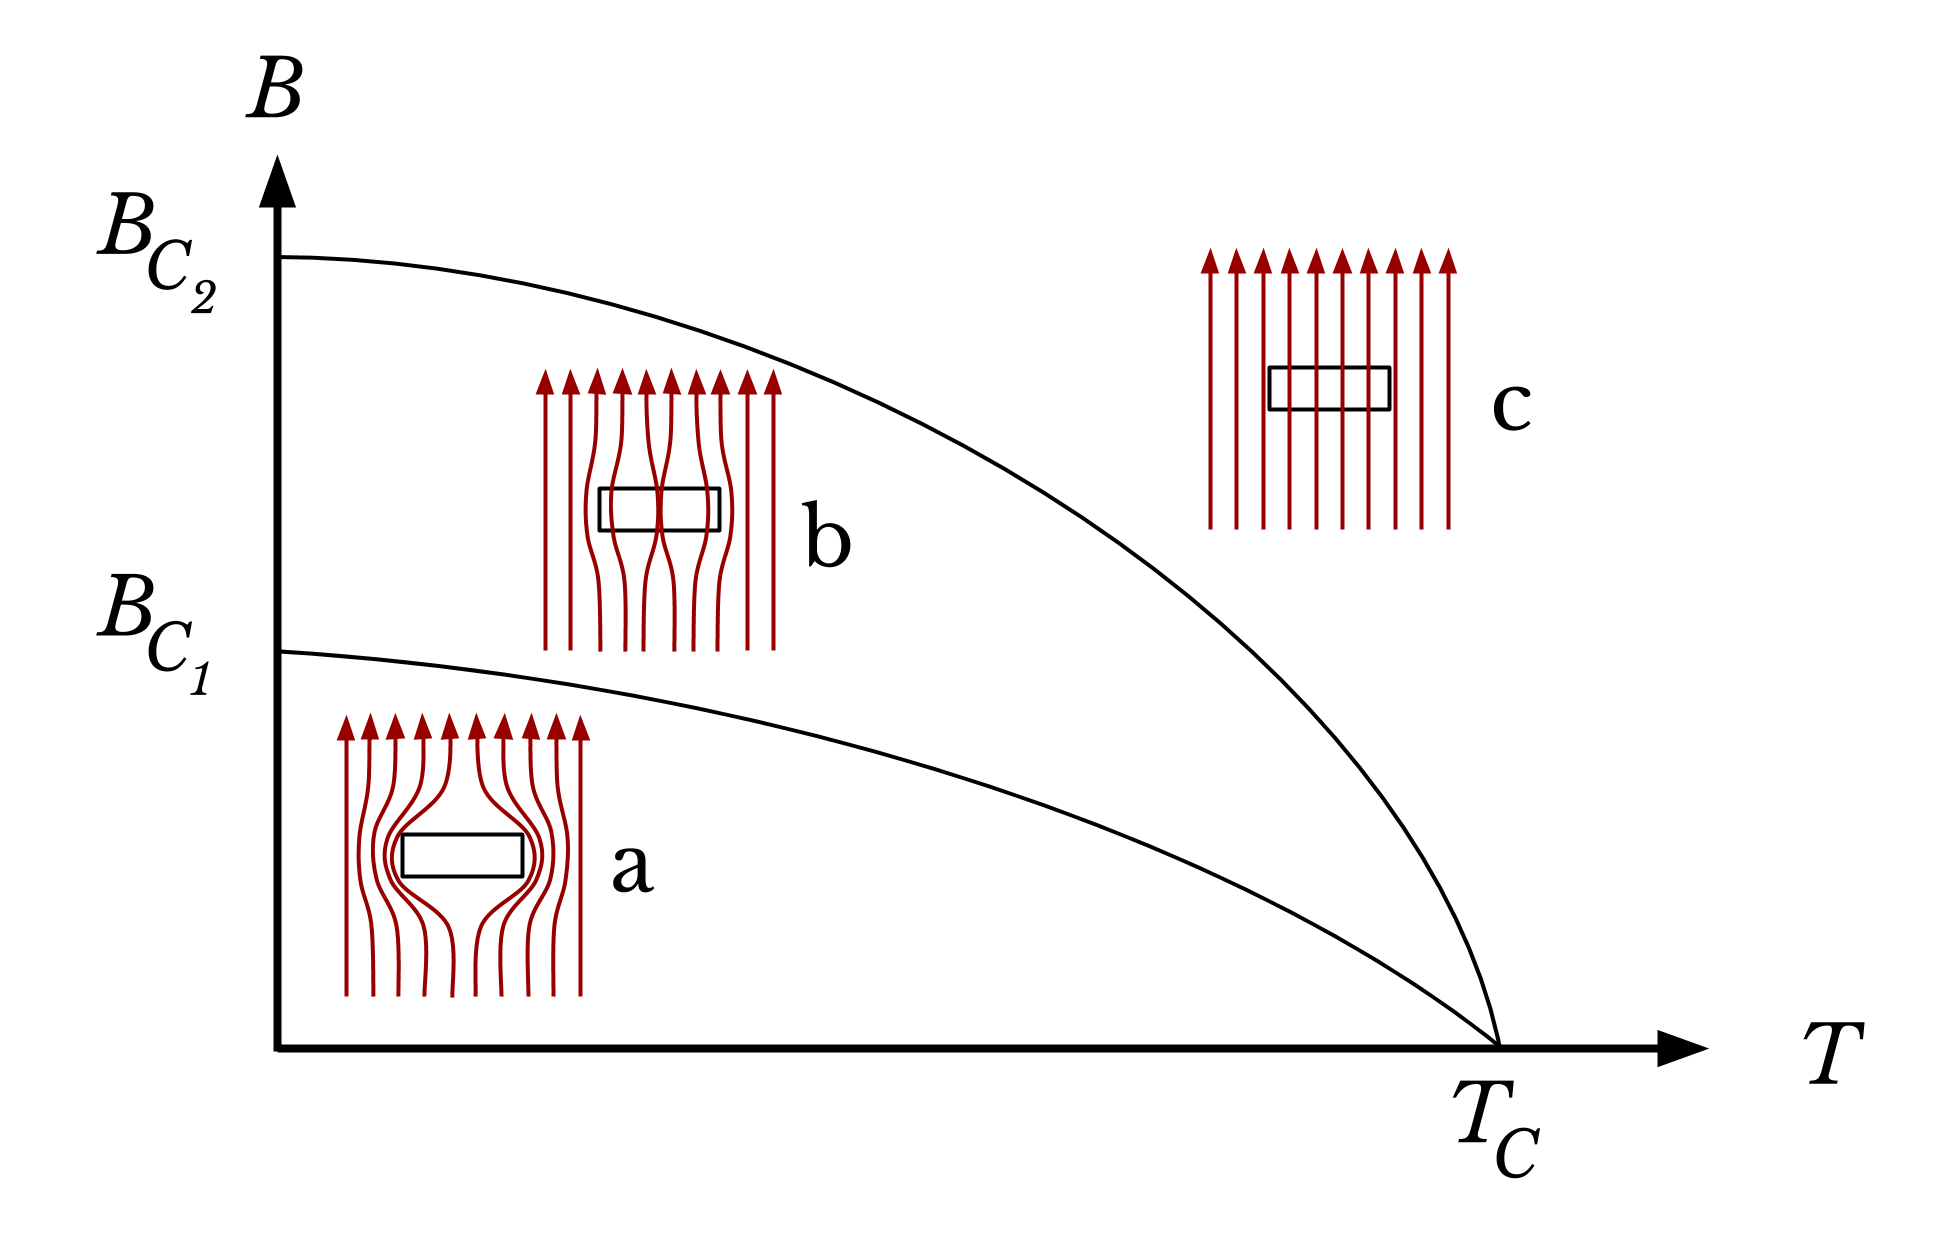
\includegraphics[width=\linewidth]{img/Superconductor_type2_phase_diagram.png}
    \caption{Phasendiagramm eines Supraleiters 2. Art.
    Die dargestellten Phasen sind (a) supraleitend, (b) Misch- oder Shubnikovphase und (c) normalleitend.
    In einem Supraleiter 1. Art existiert (b) nicht, dementsprechend gibt es dort auch nur ein kritisches Magnetfeld $B_c$.
    \refimgsource{Wikimedia}{https://commons.wikimedia.org/wiki/File:Superconductor\_interactions\_with\_magnetic\_field.png}{23.02.2022}{public domain}}
    \label{fig:superconductor type 2 phase diagram}
\end{figure}

\begin{fquestion}{Wie unterscheidet man Supraleiter?}
    Man unterscheidet zwischen Typ I ($\kappa < \frac{1}{\sqrt{2}}$, $\xi$ groß und $\lambda$ klein) und Typ II ($\kappa > \frac{1}{\sqrt{2}}$, $\xi$ klein und $\lambda$ groß) Supraleitern.
    
    Bei Typ II Supraleitern findet der Phasenübergang von der Meißner-Phase (Supraleitenden Phase) zur normalleitenden Phase über eine Mischphase (Shubnikov-Phase) statt. 
    In der Mischphase bilden sich Flussschläuche aus.
    
    Bei Typ I Supraleitern ist der Phasenübergang abrupt, siehe auch \autoref{fig:superconductor type 2 phase diagram}.
    
    Die zwei Arten unterscheiden sich auch im $B-B_a$-Diagramm (Inneres-Äußeres-Magnetfeld).
    Der Typ I Supraleiter entwickelt bei $B_a = B_c$ sprunghaft ein inneres Magnetfeld, der Typ II Supraleiter beginnt ab $B_a = B_{c1}$ dieses stetig auszubilden.
    
    \begin{center}
        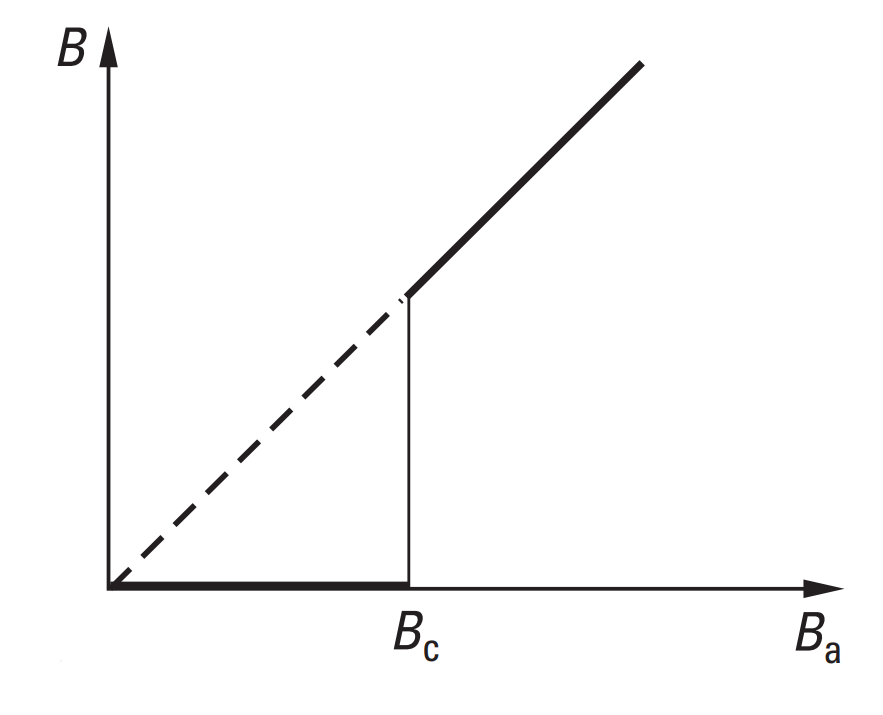
\includegraphics[width=0.4\linewidth]{img/Supraleiter_typ1.png}
        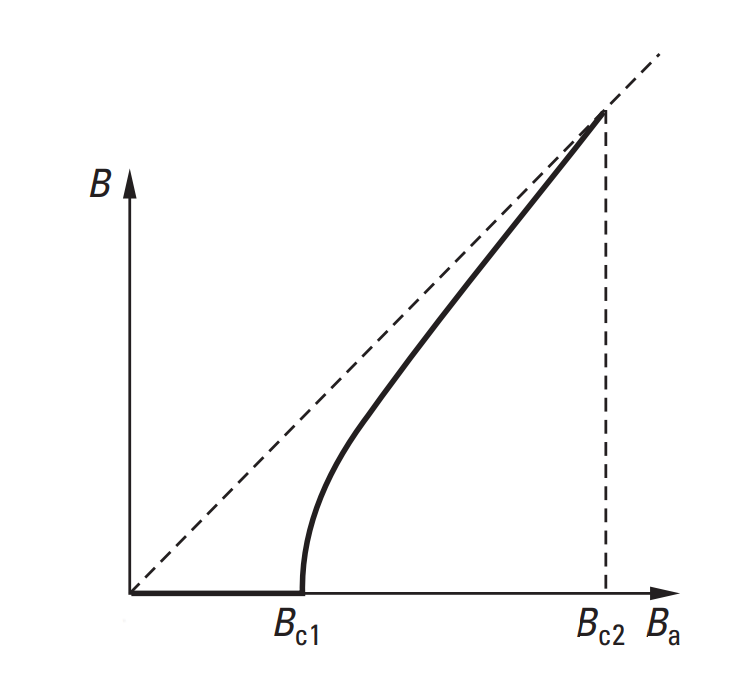
\includegraphics[width=0.4\linewidth]{img/Supraleiter_typ2.png}
    \end{center}
    \refimgsourcebook{Festkörper (Experimentalphysik, Band 6)}{Bergmann, Schäfer}{3110174855}{489f}
\end{fquestion}

\begin{figure}[!ht]
    \centering
    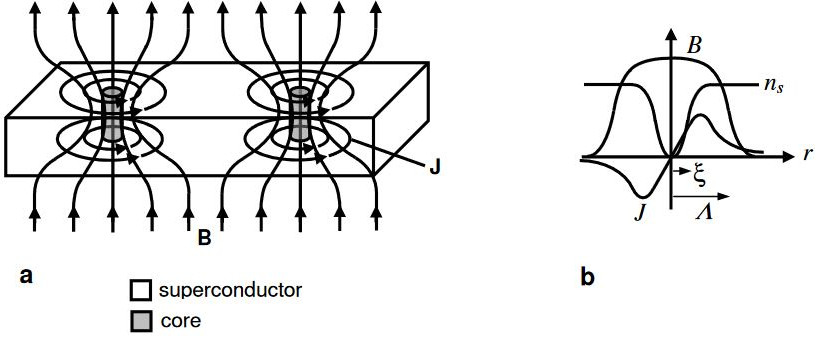
\includegraphics[width=.8\linewidth]{img/SuperconductorVortexStructure.jpg}
    \caption{Schematische Darstellung eines Flussschlauches. 
    In (a) ist das Eindringen des magnetischen Flusses über Wirbel dargestellt. 
    In (b) ist der Querschnitt eines Flussschlauches mit $B$-Feld, Kohärenzlänge $\xi$, Eindringtiefe $\Lambda$ ($\lambda$), sowie Teilchenzahl im supraleitenden Zustand $n_s$ und supraleitende Stromdichte $J$ dargestellt.
    \refimgsource{nLab}{https://ncatlab.org/nlab/files/SuperconductorVortexStructure.jpg}{17.02.2022}{Keine}}
    \label{fig:flussschlaeuche}
\end{figure}

\begin{fquestion}{Was sind Flussschläuche?}
    Flussschläuche sind die Erklärung dafür, dass bei Supraleitern 2. Art der Meißner-Ochsenfeld Effekt ab einer kritischen Temperatur bzw. einer kritischen Feldstärke nicht mehr erfüllt ist, ohne die supraleitende Eigenschaft zu verlieren.
    
    Flussschläuche sind Wirbel (Defekte) im Supraleiter, deren Inneres nicht supraleitend ist. 
    In ihrem Inneren herrscht eine Flussdichte von $\Phi_0 = \frac{h}{2e}$. 
    Eine schematische Skizze ist in \autoref{fig:flussschlaeuche} dargestellt.
\end{fquestion}

\begin{fquestion}{Was sind Beispiele für Supraleiter?}
    In der folgenden Tabelle sind verschiedene Supraleiter aufgeführt:
    \begin{center}
        \begin{tabular}{|l|lllll|}
            \hline
            Material & $T_C\, /\, \si{\kelvin}$ & $\xi\, /\, \si{\nano\metre}$ & $\lambda\, /\, \si{\nano\metre}$ & $\kappa$ &  \\
            \hline
            Al & $1.18$ & $1600$ & $50$ & $0.03$ & Typ I \\
            Pb & $7.19$ & $83$ & $39$ & $0.47$ & Typ I \\
            \hline
            Nb & $9.25$ & $40$ & $44$ & $1.1$ & Grenzfall\\
            \hline
            $\text{Nb}_3\text{Sn}$ & $18.2$ & $3.6$ & $124$ & $34$ & Typ II \\
            $\text{YBa}_2\text{Cu}_3\text{O}_{7 - \delta}$ & $90$ & $(1.5)$ & $(130)$ & $(87)$ & Typ II \\
            \hline
        \end{tabular}
    \end{center}
\end{fquestion}

% \begin{question}{Was ist ein Typ 2 Supraleiter}
%     Es kommt zu Flussschläuchen, da weder Verlust durch Verdrängung des Magnetfeldes, noch durch Unterbrechung der SL-Phase (FS sind energetisch günstiger)
% \end{question}

\begin{fquestion}{Wie kann man einen verschwindenden elektrischen Widerstand $R = 0$ messen?}
    Mit klassischen Widerstandsbrücken erhält man eine obere Schranke $R / R_n < 10^{-4}$, wobei $R$ der Widerstand in der supraleitenden und $R_n$ der in der normalleitenden Phase sind.
    Für genauere Messung benötigt man Induktionsexperimente: Etwa durch einen Stabmagneten wird in einer supraleitenden Spule ein Strom induziert, der entsprechend $ I \propto \exp \left(-R/L t\right)$ abklingt. 
    Wenn $R= 0$ ist die Abklingdauer unendlich und tatsächlich ist dadurch $R / R_n < 10^{-14}$ (über das magnetische Moment $m = I A$) messbar.
\end{fquestion}

\begin{fquestion}{Was ist die BCS-(Bardeen-Cooper-Schrieffer)-Theorie? }
    Die BCS-Theorie kann Typ I Supraleiter erklären. 
    In der BCS-Theorie werden Elektronen durch eine anziehende Wechselwirkung miteinander korreliert und bilden Cooper-Paare mit ganzzahligem Spin, unterliegen also der Bose-Einstein-Statistik. 
    
    Formell entstehen sie durch die Wechselwirkung von zwei Elektronen auf Fermi-Niveau (Streuung  an einem virtuellen Phonon), was zu einer Energieabsenkung 
    \[E \approx 2 E_F - 2 \hbar \omega_D e^{-4 / D(E_F) V_0} := 2 E_F - 2 \Delta\]
    führt.
    Für die Cooper-Paare ist es also sinnvoll in einen Grundzustand unterhalb der Fermi-Energie zu kondensieren (ist nicht das selbe wie ein Bose-Einstein-Kondensat).

    Siehe \url{https://www.thphys.uni-heidelberg.de/~wolschin/qms1920_11s.pdf}.
\end{fquestion}

\begin{fquestion}{Wie entstehen Cooper-Paare heuristisch?}
    Im Kristall entstehen Cooper-Paare durch Interaktion mit dem Gitter.
    Bewegt sich ein Elektron an Gitterplätzen vorbei, bewegen sich die positiv geladenen Atomkerne leicht in Richtung des Elektrons, wodurch eine positive Nettoladung entsteht.
    Ein Elektron entgegengesetzten Spins und Impulses interagiert mit dieser Ladung und die Elektronen werden korreliert.
\end{fquestion}

\begin{fquestion}{Wie erklären Cooper-Paare Supraleiter?}
    Der Widerstand wird durch inelastische Streuprozesse verursacht.
    Damit ein Cooper-Paar inelastisch streuen kann, muss die Energielücke $2\Delta$ überwunden werden, was bei niedrigen Temperaturen nicht möglich ist (die phänomenologische Erklärung ist hier, dass die Cooper-Paare mit $\approx \SI{100}{\nano\metre}$ weit auseinander sind und die Gitterfehler nicht spüren).
    Durch das Kondensat müssten elastische Stöße auf alle Cooper-Paare gleichzeitig wirken, wodurch die Streuung (beliebig unwahrscheinlich) nicht möglich ist.
    
    Erreicht der Strom im Leiter eine kritische Stromdichte $j_C = -e n \Delta / \hbar k_F$, können jene inelastischen Streuprozesse stattfinden und der Supraleiter bricht zusammen (das kritische Magnetfeld $B_C$ kann genau solche Ströme induzieren). 
\end{fquestion}

\begin{fquestion}{Was sind Cooper-Paare?}
    % zwei Elektronen werden durch Phononen aneinander gebunden (Ladung 2e)
    % 
    % entgegengesetzter Impuls (gleicher Betrag) und entgegengesetzter Spin (Gesamtspin S=0)
    % Erhöht oder verringert sich die Energie bei Paarbildung?
    % 
    % Cooper-Paare sind energetisch günstiger, (Zeichnung Bandlücke ??? )
    % 
    Cooper Paare sind zwei Elektronen die durch einen anziehende Wechselwirkung aneinander gebunden sind.
    Die Elektronen der Cooper-Paare tragen \textbf{entgegengesetzten Impuls}, weil dort die Wechselwirkung den größten Phasenraum (am Fermi-Rand) abdeckt und diese Paarung entsprechend am wahrscheinlichsten ist.
    Da der Ort symmetrisch gewählt wird, muss der \textbf{Spin antisymmetrisch} (entgegengesetzt sein).
    
    Die Dispersionsrelation eines Cooper-Paares ist 
    \[ E_k = \sqrt{\epsilon_k^2 + \Delta^2}\]
    wobei $\epsilon_k$ die kinetische Energie (wahlweise abzüglich des chemischen Potentials $\epsilon_k' := \epsilon_k - \mu$) der Elektronen und $\Delta$ die Bandlücke des Supraleiters ist.
    Die Cooper-Paarbildung ist entsprechend energetisch günstiger als die Bevölkerung des Fermi-Sees.
    
    Die Cooper-Paar-Kondensation führt zu einer Änderung der Zustandsdichte im Vergleich zum freien Elektronengas mit entsprechender Bandlücke:
    \begin{center}
        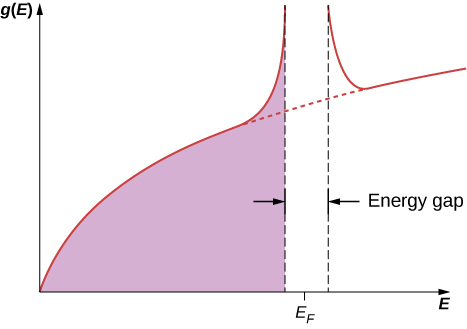
\includegraphics[width=0.5\linewidth]{img/CNX_UPhysics_42_08_EnergyGap-1.jpg}
    \end{center}
    \refimgsource{University Physics Volume 3}{https://opentextbc.ca/universityphysicsv3openstax/chapter/superconductivity/}{30.01.2022}{Creative Commons Attribution 4.0 International License}
    % 
    % Der Streuprozess, der zur Bildung von Cooper-Paaren führt ist nur durch zusätzliche kinetische Energie (etwa eine Temperatur $T \neq 0$) möglich.
    % 
    % Bindung im meV Bereich (-> thermische Energie 25 meV!)
    % Wie kann man Cooper-Paar-Bildung anschaulich erklären? 
    % 
    % Zeichnung Auslenkung des Ionengitters durch Elektron
    % Steht die Paarbildung nicht im Widerspruch zur 1. Hundschen Regel?
    % 
    % Muss wegen hohem mittleren Abstand der Elektronen nicht berücksichtigt werden
    % Wieso streuen Cooper-Paare nicht an Gitterfehlern?
    % 
    % Durchschnittlicher Abstand im Cooper-Paar ist 100 nm, also recht groß. 
    % 
    % Entweder zerbricht das Cooper-Paar an dem Gitterfehler (wenn die Energie groß genug ist) oder das Elektron streut nicht, da ansonsten gleichzeitig das Elektron 100 nm entfernt auch streuuen müsste (die Wahrscheinlichkeit quasi 0).
\end{fquestion}

\begin{fquestion}{Wie verhält sich die Wärmeleitung in der supraleitenden Phase?}
    Die Cooper-Paare tragen keine Entropie; kondensieren diese nimmt der elektronische Beitrag zur Wärmeleitung rapide ab.
    Kompensiert wird dieser Effekt durch das Ausfrieren der Gitterplätze, wodurch die Wärmeleitung im Allgemeinen steigt.
\end{fquestion}

% \begin{question}{Wie misst man, dass Phononen für die Cooper-Bindung verantwortlich sind?}
%     Der Effekt der Supraleitung ist streng mit dem Gitter verbunden, entsprechend kommen nur Phononen in Frage.    
% \end{question}

% \begin{question}{Wie misst man, dass Phononen für die Cooper-Bindung verantwortlich sind?}
%     Frequenz der Phononen ändern -> Änderung der WW ???
%     gleichen Supraleiter mit unterschiedlichen Isotopen messen -> ändert Atommassen -> ändert Frequenz -> ändert Bindung ???
% \end{question}


% \begin{question}{Welche zwei Längen sind für Supraleiter wichtig? Warum und wie erhält man diese?}
%     London'sche Eindringtiefe, Kohärenzlänge (Größenordnung ??? )
    
%     Unterscheidung von Typ I und Typ II Supraleitern (auch ??? ) anhand dieser Längen
% \end{question}

% \begin{question}{Wie kann man die Phononenanregung im Supraleitern untersuchen? }
%     Isotopeneffekt, Proportionalität der Schwingungsfrequenz zu k/m über das Hook'sche Gesetz und das Lösen der DGL des HO
% \end{question}


\begin{fquestion}{Warum ist die kritische Temperatur bei Supraleitern so klein?}
    Damit die Supraleitende Anregung messbar wird, müssen thermische Fluktuationen unter der durch die Phononanregung entstehenden Energielücke sein. 
    Entsprechend ist 
    \[T_C \propto \frac{1}{\sqrt{M}}\]
    wobei $M$ die Isotopmasse ist, entsprechend ist $T_C$ sehr klein. 
\end{fquestion}

\begin{fquestion}{Was ist der Zusammenhand zwischen der BCS- und der GLA-Theorie?}
    Der Ordnungsparameter der Ginzburg-Landau Theorie ist die Anzahl der Cooper-Paare in der BCS-Theorie.
\end{fquestion}

\begin{fquestion}{Was ist Josephson Tunneln?}
    Beim \textit{Josephson Tunneln} wird der Tunneleffekt zwischen zwei Supraleitern (getrennt durch Normalleiter oder Isolator) untersucht.
    Legt man an diese Josephson-Kontakte eine Spannung an, können die Cooper-Paar-Quasiteilchen durch die Barriere tunneln und ein Stromfluss entsteht.    
\end{fquestion}

\subsection{Deformierte Kerne}

% \begin{question}{Was sind die Ordnungs- und Brechparameter?}
%     Deformation (Ordnungsparameter) und Zahl der Valenznukleonen (Brechparameter)
% \end{question}

\begin{fquestion}{Wie kann man deformierte Kerne über Symmetriebrechung beschreiben?}
    Man betrachtet die Deformation als Ordnungsparameter und die Zahl der Valenznukleonen als Brechungsparameter im Landau-Zener-Modell.
\end{fquestion}

\subsection{Phasenübergänge}

\begin{fquestion}{Wie werden Phasenübergange charakterisiert?}
    Phasenübergänge werden nach Ehrenfest in jene $n$-ter Ordnung unterteilt.
    Dabei beschreibt $n-1$, die wie vielte Ableitung eines thermodynamischen Potentials beim Phasenübergang nicht stetig ist.
    Für $n=1$ spricht man von Phasenübergängen erster Ordnung, hier ist das Thermodynamische Potential selbst unstetig, bei $n>1$ spricht man von stetigen Phasenübergängen.
\end{fquestion}

\begin{fquestion}{Was haben Phasenübergänge 1. Klasse mit latenter Wärme zu tun?}
    Am Beispiel des schmelzenden Wassers kann man das erkennen: Hier muss man immerzu (Schmelz-)Wärme zuführen, ohne dass die Temperatur steigt. 
    Die erste Ableitung der freien Enthalpie $G$ nach $T$ (die Entropie $S$) ist entsprechend unstetig.
\end{fquestion}

\begin{figure}[!ht]
    \centering
%    \includesvg[scale=0.6]{img/Phasendiagramme.svg}
    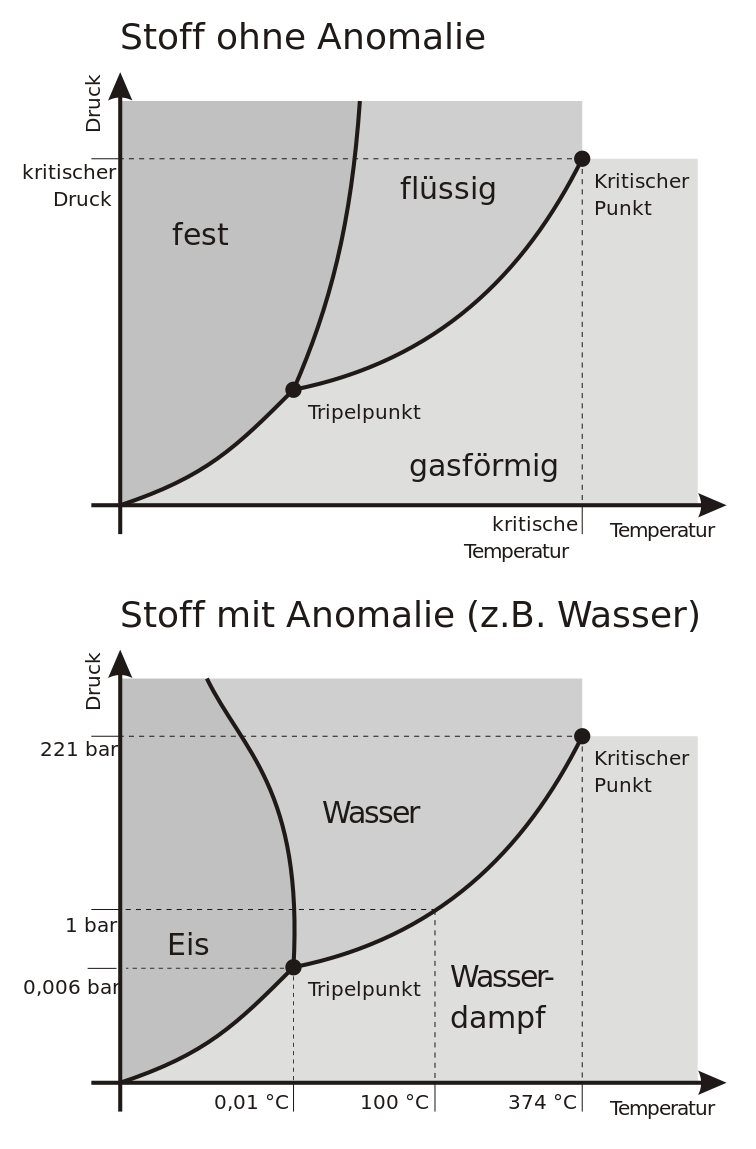
\includegraphics[width=0.6\linewidth]{img/Phasendiagramme.png}
    \caption{Phasendiagramme von Reinstoffen in der Druck-Temperatur-Ebene. Oben: ``normales'' Verhalten – die Schmelzdruckkurve zwischen fester und flüssiger Phase hat eine positive Steigung. Unten: Reinstoff mit Dichteanomalie wie etwa Wasser– die Schmelzdruckkurve zwischen fester und flüssiger Phase hat eine negative Steigung.   \refimgsource{Wikimedia}{https://commons.wikimedia.org/wiki/File:Phasendiagramme.svg}{18.01.2022}{public domain}}
\end{figure}
